\documentclass[twoside]{book}

% Packages required by doxygen
\usepackage{fixltx2e}
\usepackage{calc}
\usepackage{doxygen}
\usepackage[export]{adjustbox} % also loads graphicx
\usepackage{graphicx}
\usepackage[utf8]{inputenc}
\usepackage{makeidx}
\usepackage{multicol}
\usepackage{multirow}
\PassOptionsToPackage{warn}{textcomp}
\usepackage{textcomp}
\usepackage[nointegrals]{wasysym}
\usepackage[table]{xcolor}

% Font selection
\usepackage[T1]{fontenc}
\usepackage[scaled=.90]{helvet}
\usepackage{courier}
\usepackage{amssymb}
\usepackage{sectsty}
\renewcommand{\familydefault}{\sfdefault}
\allsectionsfont{%
  \fontseries{bc}\selectfont%
  \color{darkgray}%
}
\renewcommand{\DoxyLabelFont}{%
  \fontseries{bc}\selectfont%
  \color{darkgray}%
}
\newcommand{\+}{\discretionary{\mbox{\scriptsize$\hookleftarrow$}}{}{}}

% Page & text layout
\usepackage{geometry}
\geometry{%
  a4paper,%
  top=2.5cm,%
  bottom=2.5cm,%
  left=2.5cm,%
  right=2.5cm%
}
\tolerance=750
\hfuzz=15pt
\hbadness=750
\setlength{\emergencystretch}{15pt}
\setlength{\parindent}{0cm}
\setlength{\parskip}{3ex plus 2ex minus 2ex}
\makeatletter
\renewcommand{\paragraph}{%
  \@startsection{paragraph}{4}{0ex}{-1.0ex}{1.0ex}{%
    \normalfont\normalsize\bfseries\SS@parafont%
  }%
}
\renewcommand{\subparagraph}{%
  \@startsection{subparagraph}{5}{0ex}{-1.0ex}{1.0ex}{%
    \normalfont\normalsize\bfseries\SS@subparafont%
  }%
}
\makeatother

% Headers & footers
\usepackage{fancyhdr}
\pagestyle{fancyplain}
\fancyhead[LE]{\fancyplain{}{\bfseries\thepage}}
\fancyhead[CE]{\fancyplain{}{}}
\fancyhead[RE]{\fancyplain{}{\bfseries\leftmark}}
\fancyhead[LO]{\fancyplain{}{\bfseries\rightmark}}
\fancyhead[CO]{\fancyplain{}{}}
\fancyhead[RO]{\fancyplain{}{\bfseries\thepage}}
\fancyfoot[LE]{\fancyplain{}{}}
\fancyfoot[CE]{\fancyplain{}{}}
\fancyfoot[RE]{\fancyplain{}{\bfseries\scriptsize Generated by Doxygen }}
\fancyfoot[LO]{\fancyplain{}{\bfseries\scriptsize Generated by Doxygen }}
\fancyfoot[CO]{\fancyplain{}{}}
\fancyfoot[RO]{\fancyplain{}{}}
\renewcommand{\footrulewidth}{0.4pt}
\renewcommand{\chaptermark}[1]{%
  \markboth{#1}{}%
}
\renewcommand{\sectionmark}[1]{%
  \markright{\thesection\ #1}%
}

% Indices & bibliography
\usepackage{natbib}
\usepackage[titles]{tocloft}
\setcounter{tocdepth}{3}
\setcounter{secnumdepth}{5}
\makeindex

% Hyperlinks (required, but should be loaded last)
\usepackage{ifpdf}
\ifpdf
  \usepackage[pdftex,pagebackref=true]{hyperref}
\else
  \usepackage[ps2pdf,pagebackref=true]{hyperref}
\fi
\hypersetup{%
  colorlinks=true,%
  linkcolor=blue,%
  citecolor=blue,%
  unicode%
}

% Custom commands
\newcommand{\clearemptydoublepage}{%
  \newpage{\pagestyle{empty}\cleardoublepage}%
}

\usepackage{caption}
\captionsetup{labelsep=space,justification=centering,font={bf},singlelinecheck=off,skip=4pt,position=top}

%===== C O N T E N T S =====

\begin{document}

% Titlepage & ToC
\hypersetup{pageanchor=false,
             bookmarksnumbered=true,
             pdfencoding=unicode
            }
\pagenumbering{alph}
\begin{titlepage}
\vspace*{7cm}
\begin{center}%
{\Large Doodle }\\
\vspace*{1cm}
{\large Generated by Doxygen 1.8.14}\\
\end{center}
\end{titlepage}
\clearemptydoublepage
\pagenumbering{roman}
\tableofcontents
\clearemptydoublepage
\pagenumbering{arabic}
\hypersetup{pageanchor=true}

%--- Begin generated contents ---
\chapter{Hierarchical Index}
\section{Class Hierarchy}
This inheritance list is sorted roughly, but not completely, alphabetically\+:\begin{DoxyCompactList}
\item \contentsline{section}{Event}{\pageref{class_event}}{}
\item \contentsline{section}{Executive}{\pageref{class_executive}}{}
\item Form\begin{DoxyCompactList}
\item \contentsline{section}{Project1\+:\+:My\+Form}{\pageref{class_project1_1_1_my_form}}{}
\end{DoxyCompactList}
\item \contentsline{section}{User}{\pageref{class_user}}{}
\end{DoxyCompactList}

\chapter{Class Index}
\section{Class List}
Here are the classes, structs, unions and interfaces with brief descriptions\+:\begin{DoxyCompactList}
\item\contentsline{section}{\mbox{\hyperlink{class_event}{Event}} }{\pageref{class_event}}{}
\item\contentsline{section}{\mbox{\hyperlink{class_executive}{Executive}} }{\pageref{class_executive}}{}
\item\contentsline{section}{\mbox{\hyperlink{class_project1_1_1_my_form}{Project1\+::\+My\+Form}} \\*Summary for \mbox{\hyperlink{class_project1_1_1_my_form}{My\+Form}} }{\pageref{class_project1_1_1_my_form}}{}
\item\contentsline{section}{\mbox{\hyperlink{class_user}{User}} }{\pageref{class_user}}{}
\end{DoxyCompactList}

\chapter{Class Documentation}
\hypertarget{class_event}{}\section{Event Class Reference}
\label{class_event}\index{Event@{Event}}
\subsection*{Public Member Functions}
\begin{DoxyCompactItemize}
\item 
\mbox{\hyperlink{class_event_a5a40dd4708297f7031e29b39e039ae10}{Event}} ()
\item 
\mbox{\hyperlink{class_event_adcbdd318d0c3237e2e829549fd426d70}{Event}} (std\+::string event\+Name, std\+::string event\+Date)
\item 
void \mbox{\hyperlink{class_event_a4c6829c10c6c865759221d57a0f4a64f}{set\+Event\+Name}} (std\+::string event\+Name)
\item 
void \mbox{\hyperlink{class_event_a0fbbd58ef1341dfacea38de7795d3667}{set\+Event\+Date}} (std\+::string event\+Date)
\item 
std\+::string \mbox{\hyperlink{class_event_adf0f3e50061123d6f24200661eeb66eb}{get\+Name}} ()
\item 
std\+::string \mbox{\hyperlink{class_event_a1fb318a969eaf352d3f507b8097bd810}{get\+Date}} ()
\item 
void \mbox{\hyperlink{class_event_a099c123993ee717521ec411838d0f719}{get\+Available\+Times}} ()
\item 
void \mbox{\hyperlink{class_event_a6cf708e6ba961e2392716dd2c53d7938}{add\+User}} (\mbox{\hyperlink{class_user}{User}} u)
\item 
void \mbox{\hyperlink{class_event_aec0fa6f68332424cdfb15855765cadf3}{set\+Admin}} (std\+::string Name)
\item 
void \mbox{\hyperlink{class_event_ab573b9da583f00cd5d60934fb594e1ac}{set\+Num\+Of\+Us}} (int index, int num)
\item 
std\+::string \mbox{\hyperlink{class_event_a61903b21fd660d7ddaa126dab671a756}{get\+Admin}} ()
\item 
int \mbox{\hyperlink{class_event_a00e5f70b33801f1081ccc434a276aca5}{get\+Num\+Of\+Us}} (int index)
\item 
void \mbox{\hyperlink{class_event_a8087f742c473db50d2dda834de64ad1f}{Print}} ()
\end{DoxyCompactItemize}
\subsection*{Public Attributes}
\begin{DoxyCompactItemize}
\item 
\mbox{\Hypertarget{class_event_a78deb5cb4ee864c9ef6a90db2ad4eeab}\label{class_event_a78deb5cb4ee864c9ef6a90db2ad4eeab}} 
std\+::vector$<$ \mbox{\hyperlink{class_user}{User}} $>$ {\bfseries users}
\end{DoxyCompactItemize}
\subsection*{Private Attributes}
\begin{DoxyCompactItemize}
\item 
\mbox{\Hypertarget{class_event_ae116bf76fb01a92e000579a5a0d6f35c}\label{class_event_ae116bf76fb01a92e000579a5a0d6f35c}} 
std\+::string {\bfseries name}
\item 
\mbox{\Hypertarget{class_event_a9a93c9d38211f84cd6e347690e177f11}\label{class_event_a9a93c9d38211f84cd6e347690e177f11}} 
std\+::string {\bfseries date}
\item 
\mbox{\Hypertarget{class_event_a1c05237981f4681c77d268bb4f37183a}\label{class_event_a1c05237981f4681c77d268bb4f37183a}} 
std\+::string {\bfseries admin}
\item 
\mbox{\Hypertarget{class_event_a182ae5c5d2a1e4f5a5989a8f9f5e84b5}\label{class_event_a182ae5c5d2a1e4f5a5989a8f9f5e84b5}} 
int $\ast$ {\bfseries Num\+Of\+Us}
\end{DoxyCompactItemize}


\subsection{Constructor \& Destructor Documentation}
\mbox{\Hypertarget{class_event_a5a40dd4708297f7031e29b39e039ae10}\label{class_event_a5a40dd4708297f7031e29b39e039ae10}} 
\index{Event@{Event}!Event@{Event}}
\index{Event@{Event}!Event@{Event}}
\subsubsection{\texorpdfstring{Event()}{Event()}\hspace{0.1cm}{\footnotesize\ttfamily [1/2]}}
{\footnotesize\ttfamily Event\+::\+Event (\begin{DoxyParamCaption}{ }\end{DoxyParamCaption})}

Creates an int array to store the number of users avaliable at the cooresponding time slot 
\begin{DoxyParams}{Parameters}
{\em None} & \\
\hline
\end{DoxyParams}
\begin{DoxyReturn}{Returns}
None 
\end{DoxyReturn}
\mbox{\Hypertarget{class_event_adcbdd318d0c3237e2e829549fd426d70}\label{class_event_adcbdd318d0c3237e2e829549fd426d70}} 
\index{Event@{Event}!Event@{Event}}
\index{Event@{Event}!Event@{Event}}
\subsubsection{\texorpdfstring{Event()}{Event()}\hspace{0.1cm}{\footnotesize\ttfamily [2/2]}}
{\footnotesize\ttfamily Event\+::\+Event (\begin{DoxyParamCaption}\item[{std\+::string}]{event\+Name,  }\item[{std\+::string}]{event\+Date }\end{DoxyParamCaption})}

Stores the name and date of the event 
\begin{DoxyParams}{Parameters}
{\em Two} & strings that represent the name and date of the event \\
\hline
\end{DoxyParams}
\begin{DoxyReturn}{Returns}
None 
\end{DoxyReturn}


\subsection{Member Function Documentation}
\mbox{\Hypertarget{class_event_a6cf708e6ba961e2392716dd2c53d7938}\label{class_event_a6cf708e6ba961e2392716dd2c53d7938}} 
\index{Event@{Event}!add\+User@{add\+User}}
\index{add\+User@{add\+User}!Event@{Event}}
\subsubsection{\texorpdfstring{add\+User()}{addUser()}}
{\footnotesize\ttfamily void Event\+::add\+User (\begin{DoxyParamCaption}\item[{\mbox{\hyperlink{class_user}{User}}}]{u }\end{DoxyParamCaption})}

Adds a given user to the event 
\begin{DoxyParams}{Parameters}
{\em A} & user to be added to the event \\
\hline
\end{DoxyParams}
\begin{DoxyReturn}{Returns}
None 
\end{DoxyReturn}
\mbox{\Hypertarget{class_event_a61903b21fd660d7ddaa126dab671a756}\label{class_event_a61903b21fd660d7ddaa126dab671a756}} 
\index{Event@{Event}!get\+Admin@{get\+Admin}}
\index{get\+Admin@{get\+Admin}!Event@{Event}}
\subsubsection{\texorpdfstring{get\+Admin()}{getAdmin()}}
{\footnotesize\ttfamily std\+::string Event\+::get\+Admin (\begin{DoxyParamCaption}{ }\end{DoxyParamCaption})}

Returns the name of the admin for the event 
\begin{DoxyParams}{Parameters}
{\em None} & \\
\hline
\end{DoxyParams}
\begin{DoxyReturn}{Returns}
A string representing the name of the admin for the event 
\end{DoxyReturn}
\mbox{\Hypertarget{class_event_a099c123993ee717521ec411838d0f719}\label{class_event_a099c123993ee717521ec411838d0f719}} 
\index{Event@{Event}!get\+Available\+Times@{get\+Available\+Times}}
\index{get\+Available\+Times@{get\+Available\+Times}!Event@{Event}}
\subsubsection{\texorpdfstring{get\+Available\+Times()}{getAvailableTimes()}}
{\footnotesize\ttfamily void Event\+::get\+Available\+Times (\begin{DoxyParamCaption}{ }\end{DoxyParamCaption})}

Prints the number of users avaliable at each time slot while also saving the numbers to Num\+Of\+Us 
\begin{DoxyParams}{Parameters}
{\em None} & \\
\hline
\end{DoxyParams}
\begin{DoxyReturn}{Returns}
None 
\end{DoxyReturn}
\mbox{\Hypertarget{class_event_a1fb318a969eaf352d3f507b8097bd810}\label{class_event_a1fb318a969eaf352d3f507b8097bd810}} 
\index{Event@{Event}!get\+Date@{get\+Date}}
\index{get\+Date@{get\+Date}!Event@{Event}}
\subsubsection{\texorpdfstring{get\+Date()}{getDate()}}
{\footnotesize\ttfamily std\+::string Event\+::get\+Date (\begin{DoxyParamCaption}{ }\end{DoxyParamCaption})}

Returns the date of the event 
\begin{DoxyParams}{Parameters}
{\em None} & \\
\hline
\end{DoxyParams}
\begin{DoxyReturn}{Returns}
A string representing the date of the event 
\end{DoxyReturn}
\mbox{\Hypertarget{class_event_adf0f3e50061123d6f24200661eeb66eb}\label{class_event_adf0f3e50061123d6f24200661eeb66eb}} 
\index{Event@{Event}!get\+Name@{get\+Name}}
\index{get\+Name@{get\+Name}!Event@{Event}}
\subsubsection{\texorpdfstring{get\+Name()}{getName()}}
{\footnotesize\ttfamily std\+::string Event\+::get\+Name (\begin{DoxyParamCaption}{ }\end{DoxyParamCaption})}

Returns the name of the event 
\begin{DoxyParams}{Parameters}
{\em None} & \\
\hline
\end{DoxyParams}
\begin{DoxyReturn}{Returns}
A string representing the name of the event 
\end{DoxyReturn}
\mbox{\Hypertarget{class_event_a00e5f70b33801f1081ccc434a276aca5}\label{class_event_a00e5f70b33801f1081ccc434a276aca5}} 
\index{Event@{Event}!get\+Num\+Of\+Us@{get\+Num\+Of\+Us}}
\index{get\+Num\+Of\+Us@{get\+Num\+Of\+Us}!Event@{Event}}
\subsubsection{\texorpdfstring{get\+Num\+Of\+Us()}{getNumOfUs()}}
{\footnotesize\ttfamily int Event\+::get\+Num\+Of\+Us (\begin{DoxyParamCaption}\item[{int}]{index }\end{DoxyParamCaption})}

Takes in an index cooresponding to a time slot and returns the number of users avaliable for that time slot 
\begin{DoxyParams}{Parameters}
{\em An} & int representing the index of the time slot desired \\
\hline
\end{DoxyParams}
\begin{DoxyReturn}{Returns}
An int representing the number of users avaliable at the time slot 
\end{DoxyReturn}
\mbox{\Hypertarget{class_event_a8087f742c473db50d2dda834de64ad1f}\label{class_event_a8087f742c473db50d2dda834de64ad1f}} 
\index{Event@{Event}!Print@{Print}}
\index{Print@{Print}!Event@{Event}}
\subsubsection{\texorpdfstring{Print()}{Print()}}
{\footnotesize\ttfamily void Event\+::\+Print (\begin{DoxyParamCaption}{ }\end{DoxyParamCaption})}

Prints the number of users avaliable at each time slot 
\begin{DoxyParams}{Parameters}
{\em None} & \\
\hline
\end{DoxyParams}
\begin{DoxyReturn}{Returns}
None 
\end{DoxyReturn}
\mbox{\Hypertarget{class_event_aec0fa6f68332424cdfb15855765cadf3}\label{class_event_aec0fa6f68332424cdfb15855765cadf3}} 
\index{Event@{Event}!set\+Admin@{set\+Admin}}
\index{set\+Admin@{set\+Admin}!Event@{Event}}
\subsubsection{\texorpdfstring{set\+Admin()}{setAdmin()}}
{\footnotesize\ttfamily void Event\+::set\+Admin (\begin{DoxyParamCaption}\item[{std\+::string}]{Name }\end{DoxyParamCaption})}

Takes in the name of the admin for the event and stores it 
\begin{DoxyParams}{Parameters}
{\em A} & string representing the name of the admin for the event \\
\hline
\end{DoxyParams}
\begin{DoxyReturn}{Returns}
None 
\end{DoxyReturn}
\mbox{\Hypertarget{class_event_a0fbbd58ef1341dfacea38de7795d3667}\label{class_event_a0fbbd58ef1341dfacea38de7795d3667}} 
\index{Event@{Event}!set\+Event\+Date@{set\+Event\+Date}}
\index{set\+Event\+Date@{set\+Event\+Date}!Event@{Event}}
\subsubsection{\texorpdfstring{set\+Event\+Date()}{setEventDate()}}
{\footnotesize\ttfamily void Event\+::set\+Event\+Date (\begin{DoxyParamCaption}\item[{std\+::string}]{event\+Date }\end{DoxyParamCaption})}

Takes in a string representing the date of the event and saves it 
\begin{DoxyParams}{Parameters}
{\em A} & string representing the date of the event \\
\hline
\end{DoxyParams}
\begin{DoxyReturn}{Returns}
None 
\end{DoxyReturn}
\mbox{\Hypertarget{class_event_a4c6829c10c6c865759221d57a0f4a64f}\label{class_event_a4c6829c10c6c865759221d57a0f4a64f}} 
\index{Event@{Event}!set\+Event\+Name@{set\+Event\+Name}}
\index{set\+Event\+Name@{set\+Event\+Name}!Event@{Event}}
\subsubsection{\texorpdfstring{set\+Event\+Name()}{setEventName()}}
{\footnotesize\ttfamily void Event\+::set\+Event\+Name (\begin{DoxyParamCaption}\item[{std\+::string}]{event\+Name }\end{DoxyParamCaption})}

Takes in a string representing the name of the event and saves it 
\begin{DoxyParams}{Parameters}
{\em A} & string representing the name of the event \\
\hline
\end{DoxyParams}
\begin{DoxyReturn}{Returns}
None 
\end{DoxyReturn}
\mbox{\Hypertarget{class_event_ab573b9da583f00cd5d60934fb594e1ac}\label{class_event_ab573b9da583f00cd5d60934fb594e1ac}} 
\index{Event@{Event}!set\+Num\+Of\+Us@{set\+Num\+Of\+Us}}
\index{set\+Num\+Of\+Us@{set\+Num\+Of\+Us}!Event@{Event}}
\subsubsection{\texorpdfstring{set\+Num\+Of\+Us()}{setNumOfUs()}}
{\footnotesize\ttfamily void Event\+::set\+Num\+Of\+Us (\begin{DoxyParamCaption}\item[{int}]{index,  }\item[{int}]{num }\end{DoxyParamCaption})}

Stores the number of users avaliable at a specified time slot 
\begin{DoxyParams}{Parameters}
{\em Two} & ints representing the index of the time slot and the number of users avaliable for that time \\
\hline
\end{DoxyParams}
\begin{DoxyReturn}{Returns}
None 
\end{DoxyReturn}


The documentation for this class was generated from the following files\+:\begin{DoxyCompactItemize}
\item 
C\+:/\+Users/\+Andrew/\+Documents/\+Git\+Hub/\+Doodle/\+Project1/\+Project1/Event.\+h\item 
C\+:/\+Users/\+Andrew/\+Documents/\+Git\+Hub/\+Doodle/\+Project1/\+Project1/Event.\+cpp\end{DoxyCompactItemize}

\hypertarget{class_executive}{}\section{Executive Class Reference}
\label{class_executive}\index{Executive@{Executive}}
\subsection*{Public Member Functions}
\begin{DoxyCompactItemize}
\item 
\mbox{\hyperlink{class_executive_ad870c1d741f1f313eb0c5a8336f8af6b}{Executive}} ()
\item 
\mbox{\hyperlink{class_executive_a4ce80c499f7640b1770ade77cf56d965}{$\sim$\+Executive}} ()
\item 
void \mbox{\hyperlink{class_executive_aa6ef4869740ffb4ad00da8e03524b757}{Add\+Event}} (\mbox{\hyperlink{class_event}{Event}} E)
\item 
std\+::vector$<$ std\+::string $>$ \mbox{\hyperlink{class_executive_a4099c9d7fba8038ef79df8daddf60f1e}{check\+Aval}} (std\+::string Name)
\item 
std\+::string $\ast$ \mbox{\hyperlink{class_executive_ada44e998fdc559eba9db2f4edeef0978}{get\+All\+Events}} ()
\item 
int \mbox{\hyperlink{class_executive_a325d611b8cd579647ee657c69560f28a}{get\+Event\+Size}} ()
\item 
void \mbox{\hyperlink{class_executive_a49841644378cd9bb4b8c1cc2eee04003}{write}} ()
\item 
void \mbox{\hyperlink{class_executive_a222ab3a86234f7476e769a285bf566a4}{read}} ()
\end{DoxyCompactItemize}
\subsection*{Public Attributes}
\begin{DoxyCompactItemize}
\item 
\mbox{\Hypertarget{class_executive_a63df728eed3bdfd798e943d41d052f2d}\label{class_executive_a63df728eed3bdfd798e943d41d052f2d}} 
std\+::vector$<$ \mbox{\hyperlink{class_event}{Event}} $>$ {\bfseries events}
\item 
\mbox{\Hypertarget{class_executive_afc5d32a44263c70d0795765fc238b343}\label{class_executive_afc5d32a44263c70d0795765fc238b343}} 
\mbox{\hyperlink{class_event}{Event}} {\bfseries current\+Event}
\item 
\mbox{\Hypertarget{class_executive_a6396a22945149d9e698ac1e5d8312d93}\label{class_executive_a6396a22945149d9e698ac1e5d8312d93}} 
\mbox{\hyperlink{class_user}{User}} {\bfseries current\+User}
\end{DoxyCompactItemize}


\subsection{Constructor \& Destructor Documentation}
\mbox{\Hypertarget{class_executive_ad870c1d741f1f313eb0c5a8336f8af6b}\label{class_executive_ad870c1d741f1f313eb0c5a8336f8af6b}} 
\index{Executive@{Executive}!Executive@{Executive}}
\index{Executive@{Executive}!Executive@{Executive}}
\subsubsection{\texorpdfstring{Executive()}{Executive()}}
{\footnotesize\ttfamily Executive\+::\+Executive (\begin{DoxyParamCaption}{ }\end{DoxyParamCaption})}

Creates the object 
\begin{DoxyParams}{Parameters}
{\em None} & \\
\hline
\end{DoxyParams}
\begin{DoxyReturn}{Returns}
None 
\end{DoxyReturn}
\mbox{\Hypertarget{class_executive_a4ce80c499f7640b1770ade77cf56d965}\label{class_executive_a4ce80c499f7640b1770ade77cf56d965}} 
\index{Executive@{Executive}!````~Executive@{$\sim$\+Executive}}
\index{````~Executive@{$\sim$\+Executive}!Executive@{Executive}}
\subsubsection{\texorpdfstring{$\sim$\+Executive()}{~Executive()}}
{\footnotesize\ttfamily Executive\+::$\sim$\+Executive (\begin{DoxyParamCaption}{ }\end{DoxyParamCaption})}

Does nothing 
\begin{DoxyParams}{Parameters}
{\em None} & \\
\hline
\end{DoxyParams}
\begin{DoxyReturn}{Returns}
None 
\end{DoxyReturn}


\subsection{Member Function Documentation}
\mbox{\Hypertarget{class_executive_aa6ef4869740ffb4ad00da8e03524b757}\label{class_executive_aa6ef4869740ffb4ad00da8e03524b757}} 
\index{Executive@{Executive}!Add\+Event@{Add\+Event}}
\index{Add\+Event@{Add\+Event}!Executive@{Executive}}
\subsubsection{\texorpdfstring{Add\+Event()}{AddEvent()}}
{\footnotesize\ttfamily void Executive\+::\+Add\+Event (\begin{DoxyParamCaption}\item[{\mbox{\hyperlink{class_event}{Event}}}]{E }\end{DoxyParamCaption})}

Adds a given event to the vector that stores all the events 
\begin{DoxyParams}{Parameters}
{\em An} & event to be added to the vector \\
\hline
\end{DoxyParams}
\begin{DoxyReturn}{Returns}
None 
\end{DoxyReturn}
\mbox{\Hypertarget{class_executive_a4099c9d7fba8038ef79df8daddf60f1e}\label{class_executive_a4099c9d7fba8038ef79df8daddf60f1e}} 
\index{Executive@{Executive}!check\+Aval@{check\+Aval}}
\index{check\+Aval@{check\+Aval}!Executive@{Executive}}
\subsubsection{\texorpdfstring{check\+Aval()}{checkAval()}}
{\footnotesize\ttfamily std\+::vector$<$ std\+::string $>$ Executive\+::check\+Aval (\begin{DoxyParamCaption}\item[{std\+::string}]{Name }\end{DoxyParamCaption})}

Returns the name of the events that the given user is admin of 
\begin{DoxyParams}{Parameters}
{\em A} & string representing the name of a user \\
\hline
\end{DoxyParams}
\begin{DoxyReturn}{Returns}
A vector containing the names of the events that the given user is admin of 
\end{DoxyReturn}
\mbox{\Hypertarget{class_executive_ada44e998fdc559eba9db2f4edeef0978}\label{class_executive_ada44e998fdc559eba9db2f4edeef0978}} 
\index{Executive@{Executive}!get\+All\+Events@{get\+All\+Events}}
\index{get\+All\+Events@{get\+All\+Events}!Executive@{Executive}}
\subsubsection{\texorpdfstring{get\+All\+Events()}{getAllEvents()}}
{\footnotesize\ttfamily string $\ast$ Executive\+::get\+All\+Events (\begin{DoxyParamCaption}{ }\end{DoxyParamCaption})}

Creates a string array and stores the names of all the events currently stored in the vector 
\begin{DoxyParams}{Parameters}
{\em None} & \\
\hline
\end{DoxyParams}
\begin{DoxyReturn}{Returns}
An array of all the names of the events currently stored in the vector 
\end{DoxyReturn}
\mbox{\Hypertarget{class_executive_a325d611b8cd579647ee657c69560f28a}\label{class_executive_a325d611b8cd579647ee657c69560f28a}} 
\index{Executive@{Executive}!get\+Event\+Size@{get\+Event\+Size}}
\index{get\+Event\+Size@{get\+Event\+Size}!Executive@{Executive}}
\subsubsection{\texorpdfstring{get\+Event\+Size()}{getEventSize()}}
{\footnotesize\ttfamily int Executive\+::get\+Event\+Size (\begin{DoxyParamCaption}{ }\end{DoxyParamCaption})}

Checks the current size of the event vector and returns it 
\begin{DoxyParams}{Parameters}
{\em None} & \\
\hline
\end{DoxyParams}
\begin{DoxyReturn}{Returns}
The size of the event vector 
\end{DoxyReturn}
\mbox{\Hypertarget{class_executive_a222ab3a86234f7476e769a285bf566a4}\label{class_executive_a222ab3a86234f7476e769a285bf566a4}} 
\index{Executive@{Executive}!read@{read}}
\index{read@{read}!Executive@{Executive}}
\subsubsection{\texorpdfstring{read()}{read()}}
{\footnotesize\ttfamily void Executive\+::read (\begin{DoxyParamCaption}{ }\end{DoxyParamCaption})}

Reads the information stored in the save file and populates the events list, the users within each event, and the avaliabilites of each user 
\begin{DoxyParams}{Parameters}
{\em None} & \\
\hline
\end{DoxyParams}
\begin{DoxyReturn}{Returns}
None 
\end{DoxyReturn}
\mbox{\Hypertarget{class_executive_a49841644378cd9bb4b8c1cc2eee04003}\label{class_executive_a49841644378cd9bb4b8c1cc2eee04003}} 
\index{Executive@{Executive}!write@{write}}
\index{write@{write}!Executive@{Executive}}
\subsubsection{\texorpdfstring{write()}{write()}}
{\footnotesize\ttfamily void Executive\+::write (\begin{DoxyParamCaption}{ }\end{DoxyParamCaption})}

Stores the events list, the users, and their avaliabilities in a file so that the information is saved between program executions 
\begin{DoxyParams}{Parameters}
{\em None} & \\
\hline
\end{DoxyParams}
\begin{DoxyReturn}{Returns}
None 
\end{DoxyReturn}


The documentation for this class was generated from the following files\+:\begin{DoxyCompactItemize}
\item 
C\+:/\+Users/\+Andrew/\+Documents/\+Git\+Hub/\+Doodle/\+Project1/\+Project1/Executive.\+h\item 
C\+:/\+Users/\+Andrew/\+Documents/\+Git\+Hub/\+Doodle/\+Project1/\+Project1/Executive.\+cpp\end{DoxyCompactItemize}

\hypertarget{class_project1_1_1_my_form}{}\section{Project1\+:\+:My\+Form Class Reference}
\label{class_project1_1_1_my_form}\index{Project1\+::\+My\+Form@{Project1\+::\+My\+Form}}


Summary for \mbox{\hyperlink{class_project1_1_1_my_form}{My\+Form}}  




{\ttfamily \#include $<$My\+Form.\+h$>$}

Inheritance diagram for Project1\+:\+:My\+Form\+:\begin{figure}[H]
\begin{center}
\leavevmode
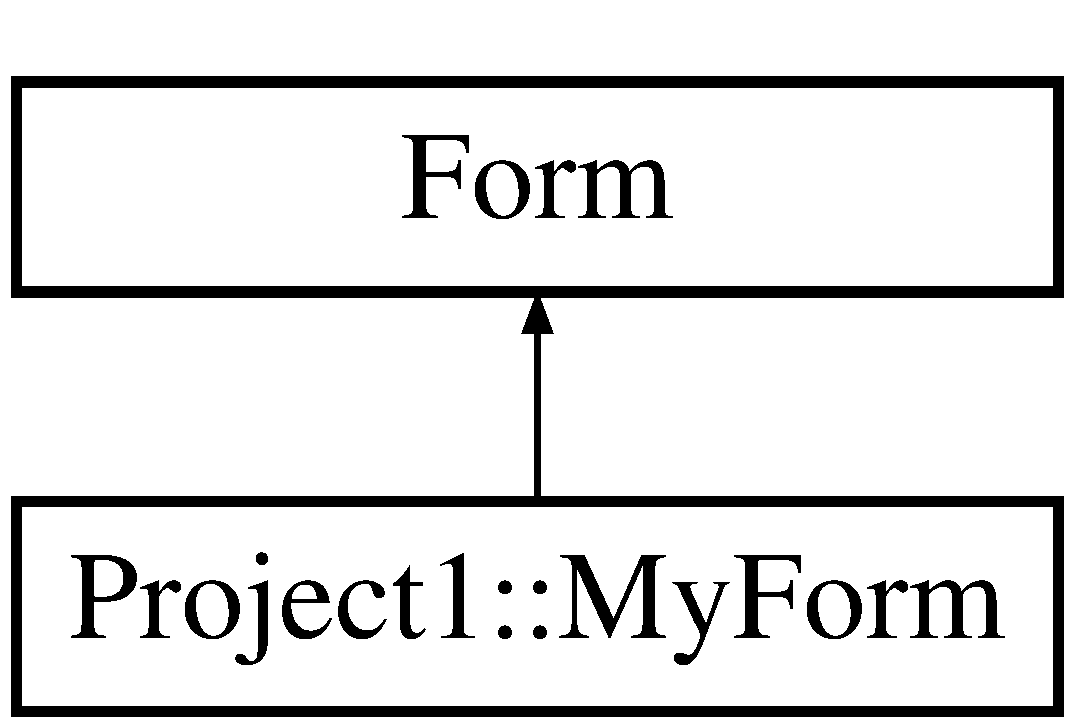
\includegraphics[height=2.000000cm]{class_project1_1_1_my_form}
\end{center}
\end{figure}
\subsection*{Public Member Functions}
\begin{DoxyCompactItemize}
\item 
\mbox{\Hypertarget{class_project1_1_1_my_form_ad665941610f014595ab9c9ca8e931765}\label{class_project1_1_1_my_form_ad665941610f014595ab9c9ca8e931765}} 
System\+::\+Void {\bfseries btn\+Submit\+Times\+\_\+\+Click} (System\+::\+Object$^\wedge$ sender, System\+::\+Event\+Args$^\wedge$ e)
\end{DoxyCompactItemize}
\subsection*{Protected Member Functions}
\begin{DoxyCompactItemize}
\item 
\mbox{\hyperlink{class_project1_1_1_my_form_a501b2b4481b72877fc73101f1d6f26be}{$\sim$\+My\+Form}} ()
\begin{DoxyCompactList}\small\item\em Clean up any resources being used. \end{DoxyCompactList}\end{DoxyCompactItemize}


\subsection{Detailed Description}
Summary for \mbox{\hyperlink{class_project1_1_1_my_form}{My\+Form}} 



\subsection{Constructor \& Destructor Documentation}
\mbox{\Hypertarget{class_project1_1_1_my_form_a501b2b4481b72877fc73101f1d6f26be}\label{class_project1_1_1_my_form_a501b2b4481b72877fc73101f1d6f26be}} 
\index{Project1\+::\+My\+Form@{Project1\+::\+My\+Form}!````~My\+Form@{$\sim$\+My\+Form}}
\index{````~My\+Form@{$\sim$\+My\+Form}!Project1\+::\+My\+Form@{Project1\+::\+My\+Form}}
\subsubsection{\texorpdfstring{$\sim$\+My\+Form()}{~MyForm()}}
{\footnotesize\ttfamily Project1\+::\+My\+Form\+::$\sim$\+My\+Form (\begin{DoxyParamCaption}{ }\end{DoxyParamCaption})\hspace{0.3cm}{\ttfamily [inline]}, {\ttfamily [protected]}}



Clean up any resources being used. 



The documentation for this class was generated from the following file\+:\begin{DoxyCompactItemize}
\item 
C\+:/\+Users/\+Andrew/\+Documents/\+Git\+Hub/\+Doodle/\+Project1/\+Project1/My\+Form.\+h\end{DoxyCompactItemize}

\hypertarget{class_user}{}\section{User Class Reference}
\label{class_user}\index{User@{User}}
\subsection*{Public Member Functions}
\begin{DoxyCompactItemize}
\item 
\mbox{\hyperlink{class_user_a4a0137053e591fbb79d9057dd7d2283d}{User}} ()
\item 
\mbox{\hyperlink{class_user_ac00b72ad64eb4149f7b21b9f5468c2b2}{$\sim$\+User}} ()
\item 
void \mbox{\hyperlink{class_user_a93c208c3a71df99ca19a1782f6d32c34}{set\+Name}} (std\+::string name)
\item 
std\+::string \mbox{\hyperlink{class_user_a3fcf5814ba0a2415862c892746585a46}{get\+User\+Name}} ()
\item 
bool \mbox{\hyperlink{class_user_ab4ba945b0431a19fef9710b16aac4bb5}{get\+Time}} (int i)
\item 
std\+::string \mbox{\hyperlink{class_user_a3b0b9cf712efbb632f920a4cc5f18925}{get\+Strings}} (int j)
\item 
void \mbox{\hyperlink{class_user_a3a637aa0a7a7b37885f2cd7dc77ecd99}{Add\+Time}} (int T)
\item 
void \mbox{\hyperlink{class_user_a70486059b5ee29b656c8331583cdd5b5}{get\+Times}} ()
\end{DoxyCompactItemize}
\subsection*{Private Attributes}
\begin{DoxyCompactItemize}
\item 
\mbox{\Hypertarget{class_user_acc74e1ba1db43cacac9c488594067060}\label{class_user_acc74e1ba1db43cacac9c488594067060}} 
std\+::string {\bfseries m\+\_\+\+Name}
\item 
\mbox{\Hypertarget{class_user_ab4a12ecb24141692e886d0d869a2ecea}\label{class_user_ab4a12ecb24141692e886d0d869a2ecea}} 
std\+::string $\ast$ {\bfseries m\+\_\+\+Strings}
\item 
\mbox{\Hypertarget{class_user_adc7849fb91c414d2ccf836e8284fd058}\label{class_user_adc7849fb91c414d2ccf836e8284fd058}} 
bool $\ast$ {\bfseries m\+\_\+\+Times}
\item 
\mbox{\Hypertarget{class_user_a2d7c25a76f9479275b46c45a3e15f300}\label{class_user_a2d7c25a76f9479275b46c45a3e15f300}} 
bool {\bfseries m\+\_\+is\+Admin}
\end{DoxyCompactItemize}


\subsection{Constructor \& Destructor Documentation}
\mbox{\Hypertarget{class_user_a4a0137053e591fbb79d9057dd7d2283d}\label{class_user_a4a0137053e591fbb79d9057dd7d2283d}} 
\index{User@{User}!User@{User}}
\index{User@{User}!User@{User}}
\subsubsection{\texorpdfstring{User()}{User()}}
{\footnotesize\ttfamily User\+::\+User (\begin{DoxyParamCaption}{ }\end{DoxyParamCaption})}

Creates the bool array m\+\_\+\+Times and sets it to false. Creates the m\+\_\+\+Strings array and populates it with the possible time slots. 
\begin{DoxyParams}{Parameters}
{\em None} & \\
\hline
\end{DoxyParams}
\begin{DoxyReturn}{Returns}
None 
\end{DoxyReturn}
\mbox{\Hypertarget{class_user_ac00b72ad64eb4149f7b21b9f5468c2b2}\label{class_user_ac00b72ad64eb4149f7b21b9f5468c2b2}} 
\index{User@{User}!````~User@{$\sim$\+User}}
\index{````~User@{$\sim$\+User}!User@{User}}
\subsubsection{\texorpdfstring{$\sim$\+User()}{~User()}}
{\footnotesize\ttfamily User\+::$\sim$\+User (\begin{DoxyParamCaption}{ }\end{DoxyParamCaption})}

Does Nothing 
\begin{DoxyParams}{Parameters}
{\em None} & \\
\hline
\end{DoxyParams}
\begin{DoxyReturn}{Returns}
None 
\end{DoxyReturn}


\subsection{Member Function Documentation}
\mbox{\Hypertarget{class_user_a3a637aa0a7a7b37885f2cd7dc77ecd99}\label{class_user_a3a637aa0a7a7b37885f2cd7dc77ecd99}} 
\index{User@{User}!Add\+Time@{Add\+Time}}
\index{Add\+Time@{Add\+Time}!User@{User}}
\subsubsection{\texorpdfstring{Add\+Time()}{AddTime()}}
{\footnotesize\ttfamily void User\+::\+Add\+Time (\begin{DoxyParamCaption}\item[{int}]{T }\end{DoxyParamCaption})}

Toggles the bool at the given index 
\begin{DoxyParams}{Parameters}
{\em An} & index representing a bool in m\+\_\+\+Times \\
\hline
\end{DoxyParams}
\begin{DoxyReturn}{Returns}
None 
\end{DoxyReturn}
\mbox{\Hypertarget{class_user_a3b0b9cf712efbb632f920a4cc5f18925}\label{class_user_a3b0b9cf712efbb632f920a4cc5f18925}} 
\index{User@{User}!get\+Strings@{get\+Strings}}
\index{get\+Strings@{get\+Strings}!User@{User}}
\subsubsection{\texorpdfstring{get\+Strings()}{getStrings()}}
{\footnotesize\ttfamily string User\+::get\+Strings (\begin{DoxyParamCaption}\item[{int}]{j }\end{DoxyParamCaption})}

Returns the string at the index passed in which represents a time slot 
\begin{DoxyParams}{Parameters}
{\em An} & int representing an index in the string array m\+\_\+\+Strings \\
\hline
\end{DoxyParams}
\begin{DoxyReturn}{Returns}
The string at the given index 
\end{DoxyReturn}
\mbox{\Hypertarget{class_user_ab4ba945b0431a19fef9710b16aac4bb5}\label{class_user_ab4ba945b0431a19fef9710b16aac4bb5}} 
\index{User@{User}!get\+Time@{get\+Time}}
\index{get\+Time@{get\+Time}!User@{User}}
\subsubsection{\texorpdfstring{get\+Time()}{getTime()}}
{\footnotesize\ttfamily bool User\+::get\+Time (\begin{DoxyParamCaption}\item[{int}]{i }\end{DoxyParamCaption})}

Returns a bool at the index passed in which represents whether the user is avaliable at that time 
\begin{DoxyParams}{Parameters}
{\em An} & int representing an index in the boolean array m\+\_\+\+Times \\
\hline
\end{DoxyParams}
\begin{DoxyReturn}{Returns}
The boolean stored at the given index 
\end{DoxyReturn}
\mbox{\Hypertarget{class_user_a70486059b5ee29b656c8331583cdd5b5}\label{class_user_a70486059b5ee29b656c8331583cdd5b5}} 
\index{User@{User}!get\+Times@{get\+Times}}
\index{get\+Times@{get\+Times}!User@{User}}
\subsubsection{\texorpdfstring{get\+Times()}{getTimes()}}
{\footnotesize\ttfamily void User\+::get\+Times (\begin{DoxyParamCaption}{ }\end{DoxyParamCaption})}

Prints the times that the user is avaliable 
\begin{DoxyParams}{Parameters}
{\em None} & \\
\hline
\end{DoxyParams}
\begin{DoxyReturn}{Returns}
None 
\end{DoxyReturn}
\mbox{\Hypertarget{class_user_a3fcf5814ba0a2415862c892746585a46}\label{class_user_a3fcf5814ba0a2415862c892746585a46}} 
\index{User@{User}!get\+User\+Name@{get\+User\+Name}}
\index{get\+User\+Name@{get\+User\+Name}!User@{User}}
\subsubsection{\texorpdfstring{get\+User\+Name()}{getUserName()}}
{\footnotesize\ttfamily string User\+::get\+User\+Name (\begin{DoxyParamCaption}{ }\end{DoxyParamCaption})}

Returns the name of the user 
\begin{DoxyParams}{Parameters}
{\em None} & \\
\hline
\end{DoxyParams}
\begin{DoxyReturn}{Returns}
The string representing the name of the user 
\end{DoxyReturn}
\mbox{\Hypertarget{class_user_a93c208c3a71df99ca19a1782f6d32c34}\label{class_user_a93c208c3a71df99ca19a1782f6d32c34}} 
\index{User@{User}!set\+Name@{set\+Name}}
\index{set\+Name@{set\+Name}!User@{User}}
\subsubsection{\texorpdfstring{set\+Name()}{setName()}}
{\footnotesize\ttfamily void User\+::set\+Name (\begin{DoxyParamCaption}\item[{std\+::string}]{name }\end{DoxyParamCaption})}

Sets the user\textquotesingle{}s name 
\begin{DoxyParams}{Parameters}
{\em String} & representing the name of the user \\
\hline
\end{DoxyParams}
\begin{DoxyReturn}{Returns}
None 
\end{DoxyReturn}


The documentation for this class was generated from the following files\+:\begin{DoxyCompactItemize}
\item 
C\+:/\+Users/\+Andrew/\+Documents/\+Git\+Hub/\+Doodle/\+Project1/\+Project1/User.\+h\item 
C\+:/\+Users/\+Andrew/\+Documents/\+Git\+Hub/\+Doodle/\+Project1/\+Project1/User.\+cpp\end{DoxyCompactItemize}

%--- End generated contents ---

% Index
\backmatter
\newpage
\phantomsection
\clearemptydoublepage
\addcontentsline{toc}{chapter}{Index}
\printindex

\end{document}
